In this section, we introduce the pricing framework that we consider in this work. We start  by giving some details on the rBergomi model proposed in \cite{bayer2016pricing}. We then derive the formula of the price of a European call option under the rBergomi model in Section \ref{sec:Option pricing under rBergomi model}. Finally, we explain  some details about the schemes that we use to simulate the dynamics of asset prices under the rBergomi model.

\subsection{The rBergomi model}\label{sec:The rBergomi model}

We consider the rBergomi model for the price process $S_t$ as defined in  \cite{bayer2016pricing}, normalized to $r=0$ ($r$ is the interest rate), which is defined by

\begin{align}\label{eq:rBergomi_model1}
	dS_t &= \sqrt{v_t} S_t dZ_t, \nonumber \\
	v_t &= \xi_0(t) \exp\left( \eta \widetilde{W}_t^H - \frac{1}{2} \eta^2 t^{2H} \right),
\end{align}
where the Hurst parameter $0 < H < 1/2$  and  $\eta>0$. We refer to $v_t$ as the variance process, and $\xi_0(t) = \expt{v_t}$ is  the forward variance curve.  Here, $\widetilde{W}^H $ is a certain Riemann-Liouville fBm
process \cite{marinucci1999alternative,picard2011representation},  defined by
\begin{align}\label{eq:Volterra process}
	\widetilde{W}_t^H = \int_0^t K^H(t-s) dW_s^1, \quad t \ge 0 \COMMA
\end{align}
where the kernel $K^H : \rset_+  \rightarrow \rset_+$ is
\begin{equation*}
 \quad K^H(t-s) = \sqrt{2H} (t-s)^{H - 1/2},\quad \forall \: 0 \le s \le t.
\end{equation*}
By construction, $\widetilde{W}^H $ is a centered, locally $(H-\epsilon)$- H\"older continuous Gaussian process with $\text{Var}\left[\widetilde{W}^H_t \right] = t^{2H}$, and a dependence structure defined by 
 \begin{equation*}
 \expt{\widetilde{W}^H_u  \widetilde{W}^H_v}=u^{2H} G\left(\frac{v}{u} \right),\quad v >u \COMMA
 \end{equation*}
 where for $x \ge 1$ and $\gamma=\frac{1}{2}-H$
 \begin{equation*}
G(x)=2H \int_{0}^1 \frac{ds}{(1-s)^{\gamma} (x-s)^{\gamma}}.
 \end{equation*}
In \eqref{eq:rBergomi_model1} and \eqref{eq:Volterra process}, $W^1, Z$ denote two \emph{correlated} standard Brownian motions with correlation $\rho \in ]-1,0]$, so that we can represent $Z$ in terms of $W^1$ as
\begin{align*}
	Z=\rho	W^1+ \bar{\rho}W^\perp = \rho W^1+\sqrt{1-\rho^2} W^\perp,
\end{align*}
where $(W^1,W^\perp)$ are two independent standard Brownian motions.
Therefore, the solution to \eqref{eq:rBergomi_model1}, with $S(0)=S_0$, can be written as 

\begin{align}\label{eq:rBergomi_model}
	S_t&= S_0  \operatorname{exp}\left( \int_{0}^{t} \sqrt{v(s)} dZ(s)- \frac{1}{2} \int_{0}^{t} v(s) ds   \right),\quad S_0>0 \nonumber\\
	v_u&=\xi_0(u) \operatorname{exp}\left( \eta \widetilde{W}_u^H- \frac{\eta^2}{2} u^{2H} \right), \quad \xi_0>0 \PERIOD
\end{align}
\begin{remark}
The rBergomi model is non-Markovian in the instantaneous variance $v_t$, that is $E\left[v_u\mid \mathcal{F}_t\right] \neq E\left[v_u\mid v_t\right]$. However, it is Markovian in the state vector by definition, that is $E\left[v_u\mid\mathcal{F}_t\right]=\xi_t(u)$.
\end{remark}
%The filtration $(\mathcal{F}_t)_{t\ge 0}$ can here be taken as the one generated by the two-dimensional Brownian motion $(W^1,W^\perp)$ under the risk neutral measure $\mathbb{Q}$, resulting in  a filtered probability space $(\Omega,\mathcal{F}, \mathcal{F}_t,\mathbb{Q})$. The stock price process $S$ is clearly then a local
%$(\mathcal{F}_t)_{t\ge 0}$-martingale and a supermartingale.  We shall henceforth use the notation $\expt{.} = E^{\mathbb{Q}}\left[. \mid \mathcal{F}_0\right]$ unless we state otherwise.


\subsection{Option pricing under the rBergomi model}\label{sec:Option pricing under rBergomi model}

We are interested in pricing European call options under the rBergomi model. Assuming $S_0 = 1$, and using the conditioning argument on the $\sigma$-algebra generated by $W^1$ (an argument first used by \cite{romano1997contingent} in the context of Markovian stochastic volatility  models), we can  show that the call price is given by

\begin{align}\label{BS_formula_rbergomi}
	C_{\text{RB}}\left( T, K \right) &= \text{E}\left[ \left(S_T - K \right)^+ \right]  \nonumber\\
	&=\expt{\expt{(S_T-K)^+ \mid \sigma(W^1(t) ,t \le T)}}\nonumber \\
	&=\text{E}\left[C_{\text{BS}}\left( S_0 = \operatorname{exp}\left(\rho \int_0^T \sqrt{v_t} dW_t^1 - \frac{1}{2}
	\rho^2 \int_0^T v_t dt\right),\ k = K, \ \sigma^2 = (1-\rho^2)
	\int_0^T v_t dt \right) \right],
\end{align}
where $C_{\text{BS}}(S_0,k,\sigma^2)$ denotes the Black-Scholes call price, for initial spot price $S_0$, strike price $k$ and volatility $\sigma^2$.

%To show \eqref{BS_formula_rbergomi}, we use the orthogonal decomposition of $S_t$ into $S_{t}^1$ and $S_{t}^2$, where
%\begin{align*}
%	S_t^1=\mathcal{E}\{ \rho \int_{0}^{t}  \sqrt{v_s} dW_s^1\}, \: S_t^2= \mathcal{E}\{ \sqrt{1-\rho^2} \int_{0}^{t}  \sqrt{v_s} dW_s^\perp  \}	,
%\end{align*}
%and $\mathcal{E}(.)$ denotes the stochastic exponential; then, if we define $\mathcal{F}_t^1= \sigma\{ W_s^1: s\le t\}$, we obtain by conditional log-normality
%\begin{align*}
%	\log S_t \mid \mathcal{F}_t^1 \sim \mathcal{N}\left( \log S_t^1-\frac{1}{2} (1-\rho^2) \int_{0}^{t} v_s ds , (1-\rho^2) \int_{0}^{t} v_s ds \right),
%\end{align*} 
%and by using the same procedure as in \cite{romano1997contingent} we obtain \eqref{BS_formula_rbergomi}.

We point out that the analytical smoothing, based on conditioning, performed in \eqref{BS_formula_rbergomi} enables us to uncover the available regularity, and hence  get a smooth, analytic integrand inside the expectation. Therefore, applying a deterministic quadrature technique such as ASGQ or QMC becomes an adequate option for computing the call price, as we will investigate later. A similar conditioning was used in \cite{mccrickerd2018turbocharging} but for variance reduction purposes only.

\subsection{Simulation of the rBergomi model}\label{sec:Simulation of the rBergomi model}

One of the numerical challenges encountered in the simulation of  rBergomi dynamics  is the computation of  $\int_{0}^{T} \sqrt{v_t} dW_t^1$ and $V=\int_{0}^{T} v_t dt$ in \eqref{BS_formula_rbergomi}, mainly because of the singularity of the Volterra kernel $K^H(s-t)$ at the diagonal $s = t$. In fact,  one needs to jointly simulate two Gaussian processes $(W_t^1, \widetilde{W}^H_t: 0 \le t \le T)$, resulting in $W^1_{t_1},\dots, W^1_{t_N}$ and $\widetilde{W}^H_{t_1},\dots, \widetilde{W}^H_{t_N}$ along a given time grid $t_1 <\dots < t_N$. In the literature, there are essentially two suggested ways to achieve this:
 \begin{enumerate}
% 	\item[i)] \textbf{Simple Euler discretization}: Euler discretization of the integral \eqref{eq:Volterra process}, defining $\widetilde{W}^H$, together with classical simulation of increments of $W^1$. This is inefficient because the integral is singular and adaptivity may not improve the scheme since the singularity moves with time. For this method, we need an $N$-dimensional random Gaussian input vector to produce one (approximate, inaccurate) sample of $W^1_{t_1},\dots, W^1_{t_N}, \widetilde{W}^H_{t_1},\dots, \widetilde{W}_{t_N}$.
 	
 	\item[i)] \textbf{Covariance based approach (exact simulation) \cite{bayer2016pricing,bayer2018short}}: $W^1_{t_1},\dots, W^1_{t_N}, \widetilde{W}^H_{t_1},\dots, \widetilde{W}_{t_N}$ together form a ($2N$)-dimensional Gaussian random vector with a computable covariance matrix, and therefore one can use Cholesky decomposition of the covariance matrix to produce exact samples of $W^1_{t_1},\dots, W^1_{t_N}, \widetilde{W}^H_{t_1},\dots, \widetilde{W}_{t_N}$ from $2 N$-dimensional Gaussian random vector as  input. This method is exact but slow. The simulation  requires $\Ordo{N^2}$ flops. Note that the offline cost is $\Ordo{N^3}$ flops.
 	
 	\item[ii)]  \textbf{The hybrid scheme of \cite{bennedsen2017hybrid}}: This scheme uses a different approach, which is essentially based on  Euler discretization  but is crucially improved by moment
 	matching for the singular term in the left point rule. It is also
 	inexact in the sense that samples produced here do not exactly have the distribution of $W^1_{t_1},\dots, W^1_{t_N}, \widetilde{W}^H_{t_1},\dots, \widetilde{W}_{t_N}$.  However they are much more accurate than the samples produced from simple Euler discretization, but much faster than method $(i)$. As in method $(i)$, in this case, we need a $2 N$-dimensional Gaussian random input vector to produce one 	sample of $W^1_{t_1},\dots, W^1_{t_N}, \widetilde{W}^H_{t_1},\dots, \widetilde{W}_{t_N}$.
 \end{enumerate} 

\subsubsection{On the choice of the simulation scheme in our approach}\label{sec: choice of simulation scheme}
The choice of the simulation scheme in our approach was based on the observed behavior of the weak rates. Through our numerical experiments (see Table \ref{table:Reference solution, using MC with $500$ time steps, of Call option price under rBergomi model, for different parameter constellation.} for the tested examples), we observe that although the hybrid and exact schemes  seem to converge asymptotically with weak error of order $\Ordo{\Delta t}$, the pre-asymptotic behavior of the weak rate is different for both schemes (we provide a short discussion of the weak error in Section \ref{sec:Weak error analysis}). As an illustration, from Figure \ref{fig:Weak_rate_set1_set_2_without_rich_hyb+chol} for Set $1$ parameter in Table \ref{table:Reference solution, using MC with $500$ time steps, of Call option price under rBergomi model, for different parameter constellation.}, the hybrid scheme  has a consistent convergence behavior in the sense that it behaves in an asymptotic manner basically right from the beginning, whereas the exact scheme does not. On the other hand, the constant  seems to be considerably smaller for the exact scheme. These two features make the hybrid scheme the  better choice   to work with in our context since our approach is based on hierarchical representations involving the use of Richardson extrapolation (see Section \ref{sec:Richardson extrapolation}).
\FloatBarrier
\begin{figure}[h!]
	\centering
	\begin{subfigure}{.4\textwidth}
		\centering
		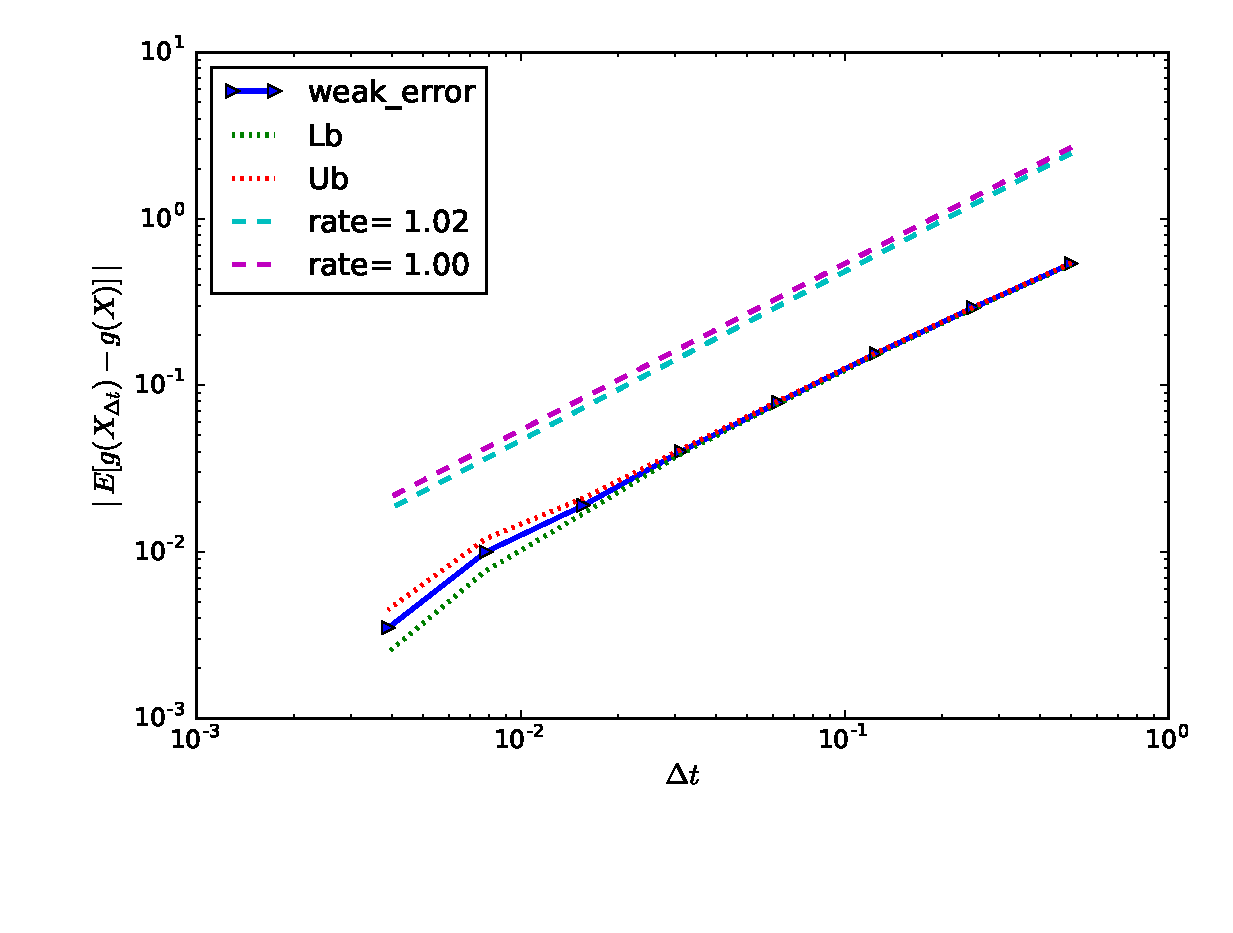
\includegraphics[width=1\linewidth]{./figures/rBergomi_weak_error_rates/without_richardson/H_007/weak_convergence_order_Bergomi_H_007_K_1_M_4_10_6_CI_relative_hybrid_non_hierarchical_non_parallel_asymptotic}
		\caption{}
		\label{fig:set1_weak_rate_hybrid}
	\end{subfigure}%
	\begin{subfigure}{.4\textwidth}
		\centering
		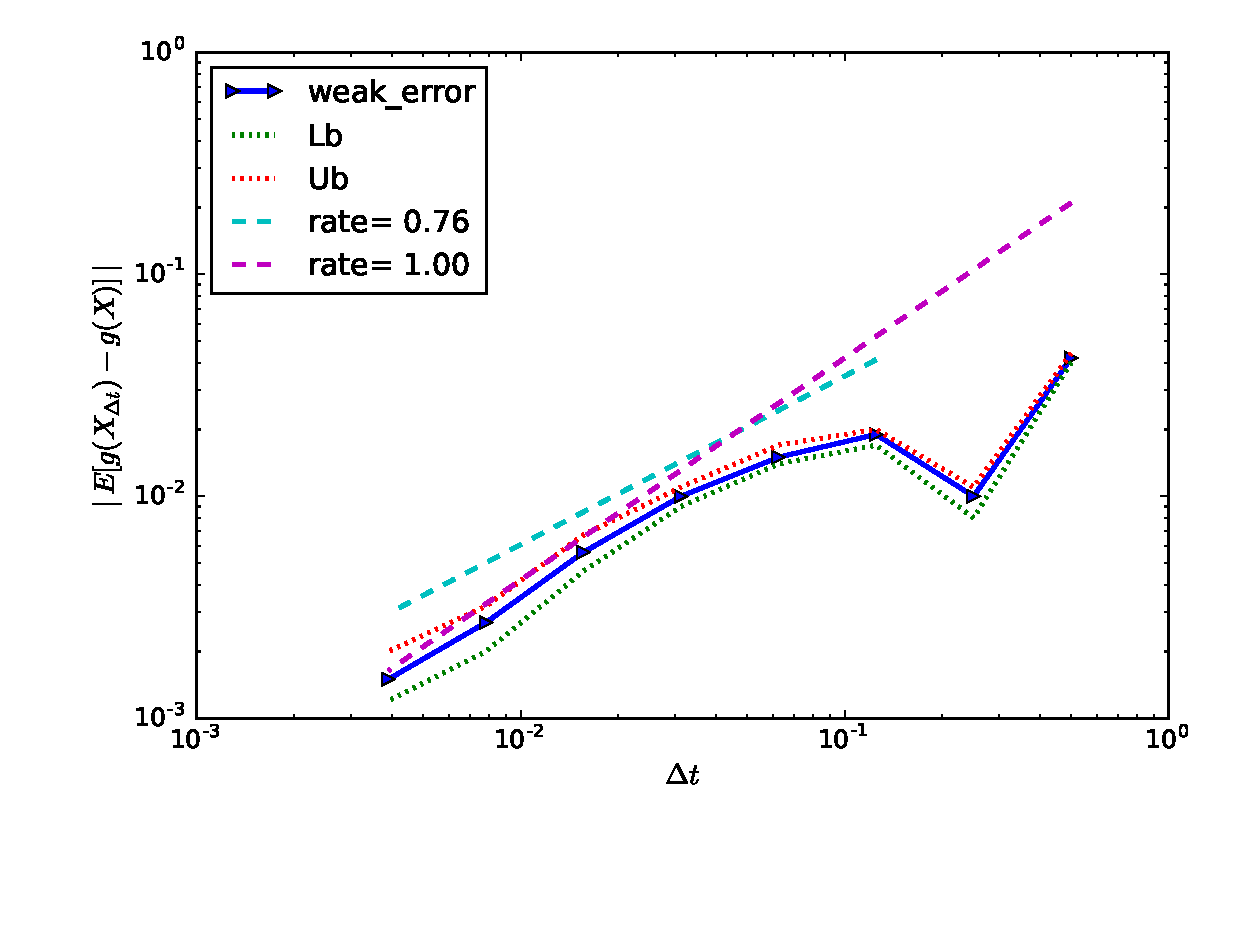
\includegraphics[width=1\linewidth]{./figures/rBergomi_weak_error_cholesky/weak_convergence_order_Bergomi_H_007_K_1_M_4_10_6_CI_relative_cholesky_non_hierarchical_non_parallel_asymptotic}
		\caption{}
		\label{fig:set1_weak_rate_exact}
	\end{subfigure}
	\caption{The convergence of the weak error $\mathcal{E}_B$,  defined in \eqref{eq: Weak_error_hyb_chol}, using MC with $6 \times 10^6$ samples, for Set $1$ parameter in Table \ref{table:Reference solution, using MC with $500$ time steps, of Call option price under rBergomi model, for different parameter constellation.}. We refer to $C_{\text{RB}}$ (as in \eqref{BS_formula_rbergomi}) for $\expt{g(X)}$, and to $C_{\text{RB}}^{N}$ (as in \eqref{BS_formula_rbergomi_2}) for $\expt{g(X_{\Delta t})}$. The upper and lower bounds are $95\%$ confidence intervals. a) With the hybrid scheme  b) With the exact scheme.}
	\label{fig:Weak_rate_set1_set_2_without_rich_hyb+chol}
\end{figure}
\FloatBarrier

\subsubsection{The hybrid scheme}\label{sec: The hybrid scheme}
As motivated in Section  \ref{sec: choice of simulation scheme}, in this work we use the hybrid scheme, which,  on an equidistant grid $\{0,\frac{1}{N},\frac{2}{N},\dots,\frac{NT}{N}\}$, is given by 
the following,
\begin{align}\label{eq:Hybrid_scheme_pre}
\widetilde{W}^H_{\frac{i}{N}} \approx \bar{W}^H_{\frac{i}{N}}&= \sqrt{2H} \left(  \sum_{k=1}^{\min(i,\kappa)} \int_{\frac{i}{N}-\frac{k}{N}}^{\frac{i}{N}-\frac{k}{N}+\frac{1}{N}} \left(\frac{i}{N}-s\right)^{H - 1/2} dW^1_s+\sum_{k=\kappa+1}^{i} \left(\frac{b_k}{N}\right)^{H - 1/2}  \int_{\frac{i}{N}-\frac{k}{N}}^{\frac{i}{N}-\frac{k}{N}+\frac{1}{N}} dW^1_s \right) \COMMA
\end{align}
which results for $\kappa=1$  in \eqref{eq:Hybrid_scheme}.
\begin{align}\label{eq:Hybrid_scheme}
\widetilde{W}^H_{\frac{i}{N}} \approx \bar{W}^H_{\frac{i}{N}}&= \sqrt{2H} \left(  W^2_i+\sum_{k=2}^{i} \left(\frac{b_k}{N}\right)^{H-\frac{1}{2}} \left(W_{\frac{i-(k-1)}{N}}^1-W_{\frac{i-k}{N}}^1\right)\right)\COMMA
\end{align}
where $N$ is the number of time steps and 
$$ b_k=\left(\frac{k^{H+\frac{1}{2}}-(k-1)^{H+\frac{1}{2} }}{H+\frac{1}{2}}\right)^{\frac{1}{H-\frac{1}{2}}} \PERIOD$$
The sum in \eqref{eq:Hybrid_scheme} requires the most computational effort in the simulation. Given that \eqref{eq:Hybrid_scheme} can be seen as discrete convolution  (see \cite{bennedsen2017hybrid}), we employ the fast Fourier transform to evaluate it, which results in  $\Ordo{N \log N}$ floating point operations.

We note that the variates $\bar{W}_0^{H},\bar{W}_1^{H},\dots,\bar{W}_{\frac{[Nt]}{N}}^{H}$ are  generated by sampling $[Nt]$ i.i.d draws from a $(\kappa+1)$-dimensional Gaussian distribution and computing a discrete convolution. We denote these pairs  of Gaussian random variables from now on by $(\mathbf{W}^{(1)},\mathbf{W}^{(2)})$. 
